Este capítulo apresenta os fundamentos em que o trabalho se apoia. A Seção~\ref{sec:info-aero} trata da informação aeronáutica, isto é, de como é publicada, que requisitos de qualidade deve atender e como os modelos de intercâmbio a representam. A Seção~\ref{sec:geo} apresenta o referenciamento linear e os conceitos de geodésia necessários para calcular comprimentos a partir de posições medidas. As Seções~\ref{sec:temporal} a~\ref{sec:adulteracao} tratam dos modelos de dados que retêm histórico: os bancos de dados temporais, o padrão \textit{event sourcing}, os registros imutáveis dos sistemas financeiros e os mecanismos de evidência de adulteração. A Seção~\ref{sec:distribuidos} discute os compromissos entre consistência e disponibilidade em sistemas distribuídos, e a Seção~\ref{sec:sintese-fund} relaciona esses fundamentos às escolhas deste trabalho.

\section{Informação aeronáutica}\label{sec:info-aero}

\subsection{Produtos, ciclo AIRAC e qualidade dos dados}\label{sec:produtos}

O Anexo~15 à Convenção de Aviação Civil Internacional e os Procedimentos para os Serviços de Navegação Aérea -- Gestão da Informação Aeronáutica (PANS-AIM) organizam a informação aeronáutica em produtos \cite{icao2018anexo15,icao2018pansaim}. Entre eles estão a Publicação de Informação Aeronáutica (AIP), com as suas emendas e suplementos, os NOTAM, as cartas aeronáuticas e, de forma crescente, os conjuntos de dados digitais. As alterações operacionalmente significativas seguem o ciclo AIRAC (\textit{Aeronautical Information Regulation and Control}). Nesse ciclo, as datas de efetividade são comuns a todos os Estados e espaçadas de 28 dias, e a publicação ocorre com antecedência mínima de 42 dias, para que os usuários possam se preparar antes da entrada em vigor. Cada emenda substitui o conteúdo afetado da edição anterior, assim, O produto publicado representa o estado dos dados na sua data de efetividade.

O Anexo~4 define o propósito de cada carta aeronáutica \cite{icao_anexo4}. A Carta de Obstáculos de Aeródromo -- Tipo~A (AOC) fornece ao operador os dados de obstáculos necessários para cumprir as limitações de desempenho na decolagem. A Carta de Aeródromo (ADC) reúne as informações que facilitam a movimentação das aeronaves no solo, entre as posições de estacionamento e a pista, além de informações operacionais essenciais do aeródromo. Os dois produtos compartilham parte dos dados, como o comprimento da pista e as distâncias declaradas. Cada um, porém, os apresenta segundo a sua finalidade e na data da sua própria emenda.

O Anexo~15 e o PANS-AIM estabelecem requisitos de qualidade para os dados aeronáuticos, que abrangem exatidão, resolução, integridade, rastreabilidade, oportunidade, completude e formato \cite{icao2018anexo15,icao2018pansaim}. Dois desses requisitos interessam diretamente a este trabalho, dentre deles a integridade, que é o grau de garantia de que um dado e o seu valor não foram perdidos nem alterados desde a sua origem ou desde uma emenda autorizada. Os dados são classificados em rotineiros, essenciais e críticos, conforme o risco associado ao seu uso incorreto. Outro requisito é a rastreabilidade, que é a capacidade de reconstituir a história, a aplicação ou a localização daquilo que se considera, e deve ser assegurada ao longo de toda a cadeia de dados. O PANS-AIM exige, além disso, consistência entre os produtos de informação aeronáutica.

Esses requisitos recaem sobre os provedores do serviço e sobre a sua cadeia de produção. O produto que chega ao usuário, contudo, apresenta os valores vigentes sem carregar a trilha que permitiria reconstituí-los.

\subsection{Distâncias declaradas}\label{sec:distancias}

O Anexo~14 define as distâncias declaradas de uma pista, que correspondem aos comprimentos disponíveis para cada fase da operação e são publicadas para cada direção de pista \cite{icao2022anexo14}. A distância disponível para corrida de decolagem (TORA, \textit{take-off run available}) é o comprimento de pista declarado disponível e adequado para a corrida no solo de uma aeronave em decolagem. A distância disponível para decolagem (TODA, \textit{take-off distance available}) acrescenta à TORA o comprimento da zona livre de obstáculos (\textit{clearway}, CWY), quando houver. De modo análogo, a distância disponível para aceleração e parada (ASDA, \textit{accelerate-stop distance available}) acrescenta à TORA o comprimento da zona de parada (\textit{stopway}, SWY). A distância disponível para pouso (LDA, \textit{landing distance available}) é o comprimento de pista declarado disponível e adequado para a corrida no solo de uma aeronave em pouso.

A zona de parada é uma área retangular além do fim da TORA, preparada para que uma aeronave possa parar em caso de decolagem abortada. Sobre a zona livre de obstáculos, a aeronave pode completar parte da subida inicial. Quando a cabeceira é deslocada, a LDA é reduzida do comprimento do deslocamento. As distâncias declaradas não são, portanto, medidas independentes. Elas resultam do comprimento da pista, das dimensões dessas áreas e da posição das cabeceiras, segundo regras normativas. A Figura~\ref{fig:distancias} mostra essas definições em uma direção de pista e a dependência de cada distância em relação às suas premissas.

\begin{figure}[htbp]
    \centering
    \begin{subfigure}{\linewidth}
        \centering
        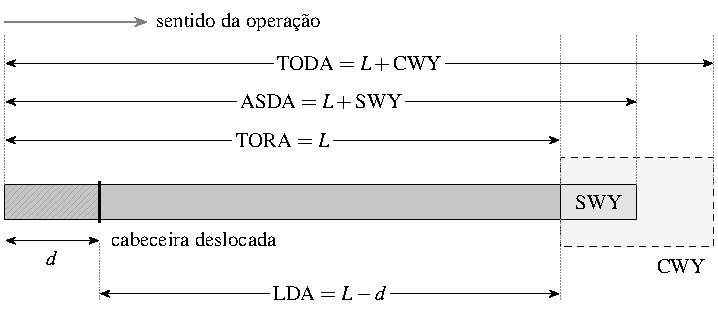
\includegraphics[page=1]{Figures/fig_distancias_declaradas.pdf}
        \caption{Esquema de uma direção de pista, fora de escala.}
        \label{fig:distancias-esquema}
    \end{subfigure}

    \bigskip
    \begin{subfigure}{\linewidth}
        \centering
        \includegraphics[page=2]{Figures/fig_distancias_declaradas.pdf}
        \caption{Dependência entre as premissas e as distâncias declaradas.}
        \label{fig:distancias-dependencia}
    \end{subfigure}

    \caption{Distâncias declaradas de uma direção de pista, segundo as definições do Anexo~14.}
    \label{fig:distancias}
    \par\smallskip{\small Fonte: o autor, a partir de \citeonline{icao2022anexo14}.}
\end{figure}

A Figura~\ref{fig:distancias} mostra essas definições em uma direção de pista e a dependência de cada distância em relação às suas premissas.

\begin{figure}[htbp]
    \centering
    \begin{subfigure}{\linewidth}
        \centering
        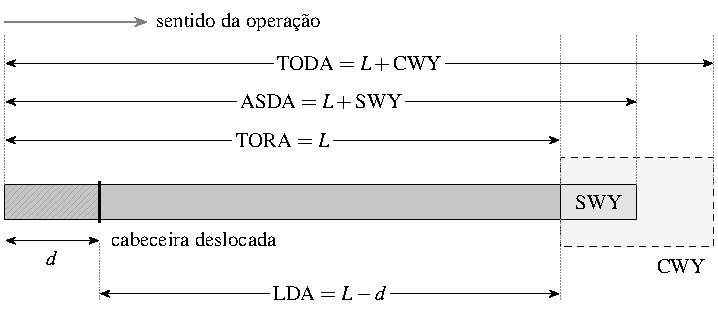
\includegraphics[page=1]{Figures/fig_distancias_declaradas.pdf}
        \caption{Esquema de uma direção de pista, fora de escala.}
        \label{fig:distancias-esquema}
    \end{subfigure}

    \bigskip
    \begin{subfigure}{\linewidth}
        \centering
        \includegraphics[page=2]{Figures/fig_distancias_declaradas.pdf}
        \caption{Dependência entre as premissas e as distâncias declaradas.}
        \label{fig:distancias-dependencia}
    \end{subfigure}

    \caption{Distâncias declaradas de uma direção de pista, segundo as definições do Anexo~14.}
    \label{fig:distancias}
    \par\smallskip{\small Fonte: o autor, a partir de \citeonline{icao2022anexo14}.}
\end{figure}

\subsection{AIXM}\label{sec:aixm}

O AIXM (\textit{Aeronautical Information Exchange Model}) é o modelo de referência para o intercâmbio digital de informação aeronáutica, desenvolvido pela EUROCONTROL e pela \textit{Federal Aviation Administration} (FAA). O modelo tem dois componentes: O primeiro é um modelo lógico em UML, com as entidades necessárias à navegação aérea, enquanto o segundo é um esquema XML baseado em GML, para a troca de dados entre sistemas \cite{eurocontrol2016aixm}. A versão 5.1.1 é a mais usada em operação.

O aspecto do AIXM mais relevante para este trabalho é o seu modelo de temporalidade \cite{eurocontrol2021temporality}. Cada \textit{Feature}, como uma pista ou uma cabeceira, tem identidade própria e é descrita por uma sequência de \textit{TimeSlices}, cada uma com um período de validade e uma interpretação. A interpretação \texttt{BASELINE} descreve o estado completo a partir de um instante, e \texttt{PERMDELTA}, uma alteração permanente. \texttt{TEMPDELTA} descreve uma alteração temporária, como a de um NOTAM, que se sobrepõe ao estado de base e expira. \texttt{SNAPSHOT}, por fim, apresenta o estado resultante em um instante, para consulta. Cada \textit{TimeSlice} traz ainda um \texttt{sequenceNumber}, que ordena as versões, e um \texttt{correctionNumber}, que identifica correções de uma versão já emitida. Os dados podem ser acompanhados de anotações em texto livre.

O AIXM tem, portanto, noção de tempo e uma disciplina de correção, mas há três aspectos que ele não garante. O primeiro é a retenção do histórico; o modelo permite representar versões e correções, mas não obriga quem publica a mantê-las, e um serviço de consulta pode devolver apenas o estado corrente. O segundo é a evidência de adulteração, já que nada no modelo permite a quem recebe os dados verificar que uma versão antiga não foi alterada depois de publicada. O terceiro é o registro das premissas e da causa de cada mudança, dessa forma, valores como as distâncias declaradas são publicados como números, sem indicação das medições que os originaram, e a razão de uma alteração, quando existe, fica em texto livre.

\subsection{Ferramentas de projeto e de SIG}\label{sec:sig}

Ferramentas de projeto, como CAD e BIM, e sistemas de informação geográfica (SIG) são as fontes mais comuns dos dados aeroportuários. O \textit{ArcGIS Aviation Airports}, da Esri, por exemplo, gera superfícies limitadoras de obstáculos de forma paramétrica, a partir do eixo e da classificação da pista, e exporta dados em AIXM \cite{esri2024}. Nessas ferramentas, o resultado do cálculo é persistido como dado primário, e é a superfície gerada, ou o desenho, que se guarda e se distribui. A relação entre esse resultado e as medições que o originaram não fica registrada, e quando existe versionamento, ele é feito sobre arquivos ou tabelas, sem registro estruturado da causa de cada alteração.

\section{Referenciamento linear e geodésia}\label{sec:geo}

\subsection{Referenciamento linear (ISO 19148)}\label{sec:iso19148}

A ISO~19148 define como expressar posições ao longo de elementos lineares, independentemente do sistema de coordenadas \cite{iso19148}. Nesse modelo, o elemento linear estabelece a direção de medição, e um referente (\textit{Referent}), ponto conhecido sobre o elemento, estabelece a origem. A posição é então dada pela distância ao longo do elemento (\textit{DistanceExpression}) e pelos afastamentos lateral e vertical em relação a ele (\textit{LateralOffsetExpression} e \textit{VerticalOffsetExpression}). Na forma geral,
\begin{equation}
    p = f(e,\, r,\, s,\, o,\, v)
    \label{eq:lrs}
\end{equation}
em que $e$ é o elemento linear, $r$ o referente, $s$ a distância ao longo do elemento, $o$ o afastamento lateral e $v$ o afastamento vertical.

O referenciamento linear é usado há décadas em rodovias e ferrovias, em que a posição de um elemento é expressa por um marco quilométrico e um afastamento. As posições, nesse modelo, não guardam coordenadas próprias, e sim uma relação com o referente. Uma nova medição do referente desloca, assim, todas as posições que dependem dele, sem que nenhuma delas precise ser reescrita.

\subsection{Distâncias sobre o elipsoide}\label{sec:geodesia}

Coordenadas geográficas são expressas em relação a um referencial geodésico. No Brasil, o referencial oficial é o SIRGAS2000 \cite{ibge2005sirgas}, que adota o elipsoide GRS80. Sobre o elipsoide, a menor distância entre dois pontos é a geodésica, cujo comprimento e cujos azimutes nas extremidades se obtêm pelo problema geodésico inverso. \citeonline{vincenty1975} resolve esse problema por iteração, com exatidão da ordem de 0,5~mm. \citeonline{karney2013} apresenta um algoritmo com exatidão próxima à da aritmética de ponto flutuante e convergência garantida em todos os casos.

A altitude também depende de uma referência. A altitude elipsoidal $h$, obtida por posicionamento por satélite, relaciona-se com a altitude ortométrica $H$, referida ao geoide, pela ondulação geoidal $N$:
\begin{equation}
    h = H + N
    \label{eq:ondulacao}
\end{equation}
As cartas de aeródromo publicam a elevação das cabeceiras e a ondulação geoidal, o que permite passar de uma referência à outra.

Projeções cartográficas, como a Universal Transversa de Mercator (UTM), representam o elipsoide em um plano à custa de deformações. Na UTM, o fator de escala vale 0,9996 no meridiano central de cada fuso e varia com o afastamento a ele. O norte da quadrícula, além disso, não coincide com o norte verdadeiro, e a diferença entre eles é a convergência meridiana. Distâncias e azimutes medidos sobre a projeção diferem, portanto, dos medidos sobre o elipsoide, e a diferença varia com a posição.

Um comprimento calculado sobre o elipsoide tampouco coincide com o comprimento medido sobre o terreno, e duas reduções os relacionam. A primeira é a de altitude. Uma distância horizontal $D_h$, medida à altitude $h$, corresponde no elipsoide a
\begin{equation}
    D_0 = D_h \frac{R}{R + h} \approx D_h \left(1 - \frac{h}{R}\right)
    \label{eq:reducao-altitude}
\end{equation}
em que $R$ é o raio de curvatura da Terra no local. A segunda é a de inclinação. Entre dois pontos com desnível $\Delta z$ e distância horizontal $L$, a distância inclinada excede a horizontal em aproximadamente
\begin{equation}
    \Delta L \approx \frac{\Delta z^2}{2L}
    \label{eq:reducao-inclinacao}
\end{equation}
Um produto que publique comprimentos precisa, portanto, declarar a convenção adotada. Sem essa declaração, dois valores corretos para a mesma pista podem diferir apenas por convenção.

\section{Dados temporais}\label{sec:temporal}

\subsection{Tempo de validade e tempo de transação}\label{sec:bitemporal}

A retenção do histórico de um banco de dados, e não apenas do seu estado corrente, é estudada há décadas na área de bancos de dados temporais. \citeonline{snodgrass2000} distingue dois eixos de tempo. O tempo de validade corresponde ao período em que um fato é verdadeiro no mundo, e o tempo de transação, ao instante em que o fato foi registrado no banco. Um banco que mantém os dois eixos é chamado bitemporal.

A distinção tem consequências diferentes conforme o domínio. Em uma transação financeira, o lançamento registrado constitui o próprio fato para fins contábeis, e o saldo de uma conta não descreve nenhum objeto independente do sistema. Os dados aeronáuticos, ao contrário, descrevem objetos físicos que existem independentemente da sua representação. Uma pista existe antes de ser medida ou publicada, e a sua medição pode ser registrada dias ou meses depois de realizada, além de poder estar incorreta.

Considere uma pista cujo comprimento sempre foi de 2500~m, mas que foi publicada durante anos com o valor de 2600~m. Quando o erro é identificado, registra-se uma correção, e o histórico admite duas leituras. Com apenas o tempo de transação, o sistema informa que o valor publicado era de 2600~m até a data da correção, o que permite reconstruir o que foi oficialmente informado em cada instante. Com os dois eixos, o sistema representa, ao mesmo tempo, que a pista sempre teve 2500~m e que o registro informava 2600~m até determinada data. A primeira leitura atende à auditoria documental, enquanto a segunda permite também relacionar ocorrências passadas a uma condição que só foi reconhecida depois.

\subsection{Event sourcing e CQRS}\label{sec:event-sourcing}

\citeonline{fowler2005} descreve o padrão \textit{event sourcing}, que leva a retenção do histórico ao seu limite, e nele, o estado não é gravado, mas derivado da sequência de eventos que o produziu. Cada alteração é um evento acrescentado a um registro em que só se escreve, e o estado em qualquer instante é obtido reprocessando os eventos até ele.

O padrão costuma vir acompanhado da segregação entre comandos e consultas (CQRS, \textit{Command Query Responsibility Segregation}), descrita por \citeonline{young2010}. O lado da escrita valida os comandos e registra os eventos. O lado da leitura monta, a partir deles, tantos modelos de consulta quantos forem necessários, todos descartáveis e reconstruíveis. \citeonline{kleppmann2017} mostra como esse modelo, em que um registro ordenado é a fonte da verdade e os demais dados são derivados dele, sustenta sistemas de dados de grande porte.

\section{Registros imutáveis em sistemas financeiros}\label{sec:financeiro}

O registro de eventos imutáveis é a base de sistemas financeiros em produção, nos quais a exigência de auditoria é antiga e o volume de operações é muito maior que o da informação aeronáutica. Em um livro-razão, nenhum lançamento é apagado, um erro é corrigido por um lançamento de estorno e o saldo é derivado dos lançamentos \cite{helland2016}. Dessa forma, empresas de pagamento aplicam esse princípio diretamente, como mostram os registros de movimentação de dinheiro da Stripe \cite{ganelin2024} e da Square \cite{strzalkowski2019}.

\citeonline{fowler2011} descreve o núcleo da LMAX, uma bolsa de negociação de varejo. Toda a lógica de negócio é executada em memória, em uma única \textit{thread}, e processa cerca de seis milhões de pedidos por segundo, o estado, no entanto, não é persistido diretamente. Cada evento de entrada é gravado em um diário (\textit{journal}) antes de ser processado, e, em caso de falha, o estado é reconstruído reprocessando esses eventos a partir do último \textit{snapshot}. O caso mostra que a reconstrução do estado a partir de eventos é um mecanismo de operação, e não apenas de laboratório, e que o seu custo de escrita não é impeditivo.

Nenhum dos dois casos trata, porém, da evidência de adulteração e não permitem que um terceiro verifique que eles não foram alterados. Essa garantia vem de outra linha de trabalho, tratada a seguir.

\section{Evidência de adulteração}\label{sec:adulteracao}

\citeonline{haber1991} propõem encadear registros por funções de \textit{hash}. Cada registro inclui o \textit{hash} do anterior, de modo que alterar qualquer um deles invalida todos os elos seguintes. A mesma ideia sustenta os bancos de dados de \textit{ledger}, que guardam o histórico de forma verificável. \citeonline{antonopoulos2021} descrevem o SQL Ledger, do Azure SQL Database, que mantém as tabelas comuns do banco, mas encadeia criptograficamente cada transação. O sistema também publica resumos (\textit{digests}) que permitem verificar, posteriormente, que nada foi alterado.

Esse mecanismo tem um limite. A cadeia detecta alterações pontuais, mas não a reescrita completa do registro por quem o controla, que produz uma nova sequência internamente coerente. Essa reescrita só é detectada se um resumo anterior do registro, como o \textit{hash} do último elo (a cabeça da cadeia), tiver sido guardado fora do sistema, na forma de uma âncora externa. É por essa razão que o SQL Ledger publica os seus resumos em armazenamento externo e imutável.

\section{Consistência e disponibilidade em sistemas distribuídos}\label{sec:distribuidos}

Quando os dados são replicados para vários leitores, surge um compromisso conhecido. \citeonline{brewer2000} formula o teorema CAP, que \citeonline{gilbert2002} demonstram formalmente. Segundo o teorema, um sistema distribuído, diante de uma partição da rede, precisa escolher entre consistência e disponibilidade. Ou responde sempre, ainda que com dados possivelmente desatualizados, ou responde sempre de forma consistente, ainda que às vezes deixe de responder.

\citeonline{kleppmann2017} mostra que esse compromisso pode ser resolvido de forma diferente em cada parte de um sistema construído sobre um registro ordenado. A escrita pode ser centralizada em um único ponto, que impõe a ordem total dos eventos, enquanto a leitura é distribuída entre consumidores que mantêm as suas próprias cópias derivadas. A transferência dos eventos do banco para os consumidores é feita por captura de mudanças (\textit{change data capture}, CDC), seja pela leitura do registro do banco, seja por uma tabela de saída (\textit{outbox}) gravada na mesma transação. Cada consumidor guarda apenas a sua posição de leitura. Como o registro só cresce, um consumidor atrasado conhece um prefixo do registro, e nunca uma versão divergente dele.

\section{Síntese}\label{sec:sintese-fund}

Os fundamentos apresentados delimitam o espaço em que este trabalho se situa. A informação aeronáutica já dispõe de requisitos de integridade e rastreabilidade e de um modelo de intercâmbio com noção de tempo, mas nenhum dos dois assegura que o histórico, as premissas e a causa de cada alteração cheguem ao usuário junto com os dados. As distâncias declaradas, por sua vez, decorrem de regras do Anexo~14 aplicadas a posições e dimensões, o que as torna candidatas naturais a valores calculados, e não armazenados. O referenciamento linear da ISO~19148 e a geodésia sobre o elipsoide oferecem os meios para registrar posições por dependência e para calcular comprimentos sob uma convenção explícita.

Dos modelos que retêm histórico, este trabalho adota o \textit{event sourcing} e a separação entre escrita e leitura, com o tempo de transação como única linha do tempo e a bitemporalidade como extensão possível. Dos sistemas financeiros, adota o princípio do livro-razão, em que nada se apaga e toda correção é um novo registro. Da linha de evidência de adulteração, adota o encadeamento por \textit{hash}, com a cadeia linear pelo pequeno volume do domínio, e reconhece o limite que só uma âncora externa supera. A discussão sobre sistemas distribuídos, por fim, fundamenta a escolha de privilegiar a consistência na escrita e a disponibilidade na leitura. O Capítulo~\ref{chap:metodologia} parte desses fundamentos para definir os requisitos do artefato e o método pelo qual ele é avaliado.
